\newpage
\section{Ergebnisse}
In diesem Kapitel werden die zentralen Ergebnisse der Arbeit präsentiert.
Im Mittelpunkt steht der entwickelte \acs{aas}-Demonstrator, der die prototypische Umsetzung des digitalen Zwillings des Abfüll- und Verschließmoduls der robocell-Linie zeigt.
Darauf folgt die Analyse des eingesetzten Autoencoder-Modells zur Anomalieerkennung sowie die Vorstellung der beiden Anwendungsfälle \acs{dpp} und automatisierte Generierung der \acs{aas}.
Abschließend werden die im Projekt eingesetzten Softwarelösungen und Tools evaluiert.

\subsection{AAS-Demonstrator für die robocell}
Der \acs{aas}-Demonstrator basiert auf dem standardisierten Konzept der \acs{aas}.
Als zentrale Laufzeitumgebung kommt die Eclipse BaSyx-Plattform zum Einsatz, während für die Datenanbindung standardisierte Protokolle wie OPC~UA verwendet werden.
Neben der Haupt-AAS der robocell-Maschine sind auch exemplarische AAS untergeordneter Komponenten integriert, wodurch eine modulare und hierarchisch aufgebaute digitale Repräsentation entsteht.

Im weiteren Verlauf wird zunächst die Architektur des Gesamtsystems vorgestellt.
Sie dient der Verwaltung und Bereitstellung aller modellierten \acs{aas} und bildet die Grundlage für die dynamische Erweiterung um Echtzeit- und Zeitreihendaten.
Anschließend werden die im Demonstrator abgebildeten Aspekte der Maschine beschrieben, gegliedert in statische und dynamische Submodelle.
Den Abschluss bildet eine kurze Reflexion über zentrale Herausforderungen, die während der Implementierung aufgetreten sind.

\subsubsection{Systemarchitektur}
Die eingesetzte Architektur besteht aus mehreren Komponenten, die gemeinsam einen aktiven digitalen Zwilling im Sinne einer Typ-2-\acs{aas} ermöglichen.
Sie basiert vollständig auf containerisierten Diensten, die innerhalb einer gemeinsamen Docker-Umgebung über ein gemeinsames Netzwerk miteinander kommunizieren.
Dadurch entsteht eine modulare, skalierbare Infrastruktur, die sich flexibel erweitern und an veränderte Anforderungen anpassen lässt.

Als zentrale Plattform zur Bereitstellung und Verwaltung der \acs{aas} dient Eclipse BaSyx.
Ursprünglich war der Einsatz des AASX Server Blazor vorgesehen, dieser wurde jedoch frühzeitig durch BaSyx ersetzt, da sie eine deutlich flexiblere und funktionsreichere Umgebung für die Umsetzung digitaler Zwillinge bietet.
Abbildung~\ref{fig:BaSyxArchitektur} zeigt den Aufbau des zugrundeliegenden Systems.

\begin{figure}[htbp]
    \centering
        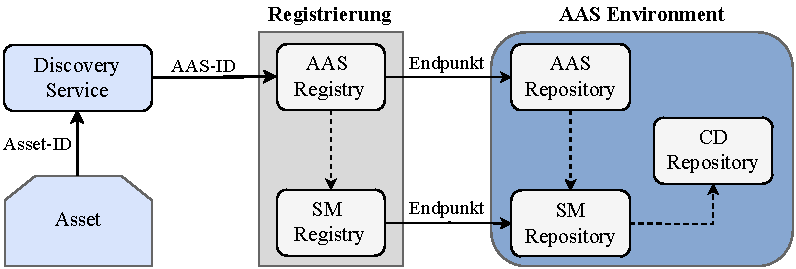
\includegraphics[width=1\textwidth]{Bilder/Ergebnisse/Systemarchitektur/BaSyx.pdf}
    \caption{???}
    \label{fig:BaSyxArchitektur}
\end{figure}

Der Discovery Service übernimmt die Auflösung einer Asset-ID (globalAssetId) in die zugehörige \acs{aas}-ID und ermöglicht so das gezielte Auffinden einer \acs{aas} im Gesamtsystem. 
Die Registries dienen als Verzeichnisse aller registrierten \acs{aas} und Submodelle einschließlich ihrer Endpunkte innerhalb der \acs{aas} Environment, wobei die \acs{aas} Registry optional auch Referenzen auf die Submodel Registry (SM Registry) enthalten kann. 

Die \acs{aas} Environment selbst beherbergt die eigentlichen Inhalte und ist in drei Repositories gegliedert. 
Das AAS Repository verwaltet die \acs{aas} einschließlich Asset-Metadaten und Referenzen auf Submodelle. 
Das Submodel Repository (SM Repository) speichert die Submodelle mit ihren jeweiligen Inhalten und Referenzen auf Concept Descriptions. 
Das \acs{cd} Repository enthält die zugehörigen semantischen Beschreibungen. 

Alle Komponenten verfügen über eine standardisierte REST-API, die sowohl anderen Systemen als auch den Komponenten selbst einen einheitlichen Zugriff auf ihre Inhalte ermöglicht. 
Zudem sind sie an eine gemeinsame MongoDB angebunden, in der sämtliche Daten persistent gespeichert werden.

\begin{figure}[htbp]
    \centering
        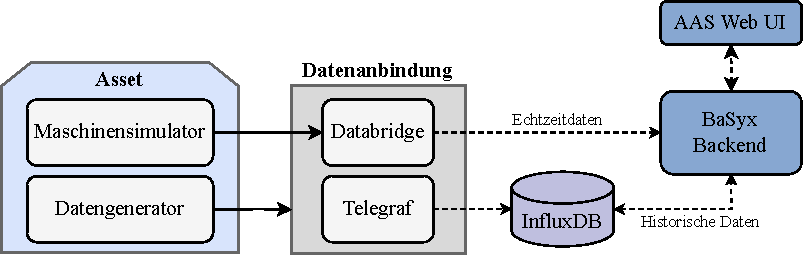
\includegraphics[width=1\textwidth]{Bilder/Ergebnisse/Systemarchitektur/DynamischeErwweiterung.pdf}
    \caption{???}
    \label{fig:BaSyxArchitektur}
\end{figure}

Die dynamische Erweiterung des Demonstrators ergänzt die BaSyx-Kernarchitektur um eine Anbindung von Echtzeit- und historischen Daten. 
Abbildung~\ref{fig:DynamischeErweiterung} zeigt den Aufbau der zusätzlichen Komponenten und deren Zusammenspiel mit dem bestehenden System.

Die Datenquellen bilden der Maschinensimulator sowie der Datengenerator, die sowohl Echtzeitdaten als auch historische Daten erzeugen. 
Diese werden über eine Datenanbindung (Data Bridge) in das System eingespeist. 
Für die Erfassung und Zwischenspeicherung von Echtzeitdaten kommt \textit{Telegraf} zum Einsatz, während die Zeitreihendaten in einer \textit{InfluxDB} persistiert werden. 
Das BaSyx Backend greift auf diese Daten zu und stellt sie in den entsprechenden Submodellen der \acs{aas} bereit. 
Über das AAS Web UI können die aktuellen Werte und historischen Verläufe visualisiert und analysiert werden.
% Ein wesentlicher Vorteil der gewählten Architektur besteht darin, dass sich die AAS Web UI jederzeit durch alternative Frontends oder zusätzliche Services ersetzen lässt.
% Dadurch können sowohl eigene Anwendungen als auch externe Softwarelösungen flexibel integriert werden.
% Im Rahmen dieser Arbeit wurde beispielsweise alternativ der Mnestix Browser eingesetzt, der eine vergleichbare Funktionalität wie die AAS Web UI bietet \cite{Quelle}.
% Eine detaillierte Evaluierung  folgt in Kapitel~\ref{ref}.

% -----------------

% \subsubsection{Stammdaten}
% \subsubsection*{Typenschild}
% \vspace{-0.5em}

% Das Submodell Typenschild bildet die zentrale Identifikationsstelle innerhalb des Demonstrators und entspricht funktional einem physischen Typenschild. 
% Es enthält grundlegende Informationen wie Hersteller, Seriennummer oder Produkttyp. 
% Auch bei Maschinen von groninger sind solche Typenschilder vorhanden, jedoch meist reduziert auf die wichtigsten Angaben.

% Die digitale Variante innerhalb der \acs{aas} erlaubt eine erweiterte Darstellung dieser Informationen, die sowohl maschinenlesbar als auch interoperabel sind. 
% Dazu zählen beispielsweise Softwareversionen, Zertifikate, Logos, Kontaktinformationen oder weitere produktspezifische Angaben, die über ein physisches Typenschild hinausgehen. 

% Das Typenschild zählt zu den wichtigsten Submodellen und ist daher auch als Plugin in der AAS Web UI verfügbar. 
% Dort ist es unterteilt in Produktinformationen und Herstellerinformationen. 
% In Abbildung~\ref{fig:Typenschild} ist exemplarisch der Herstellerbereich des Plugins dargestellt.

% \begin{figure}[htbp]
%     \centering
%         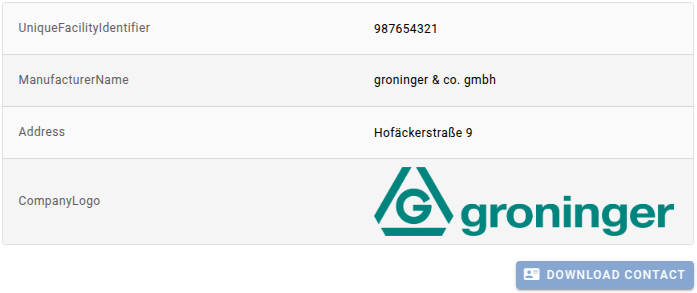
\includegraphics[width=1\textwidth]{Bilder/Ergebnisse/StatischeDaten/Typenschildisualisierung.png}
%     \caption{Metadatenstruktur im Submodell Dokumentation}
%     \label{fig:Typenschild}
% \end{figure}

% \subsubsection*{Technische Daten}
% \vspace{-0.5em}

% Analog zur in Kapitel \ref{chap:ErstellenvonSubmodelTemplates} beschriebenen Vorgehensweise wurde das generische \acs{smt} TechnicalData \cite{SpezifikaitonTechnischeDaten} an die spezifischen Anforderungen der Maschine angepasst. 
% Dabei wurden die wichtigsten Eigenschaften zusammengeführt und in eigenen \acs{smc} strukturiert. 
% Zu den erfassten Daten zählen allgemeine Informationen, Produktionsmedien, Umgebungsbedingungen sowie, wie auch in Abbildung xy ersichtlich, elektrische Daten und der Verarbeitungsbereich.

% \begin{figure}[htbp]
%     \centering
%         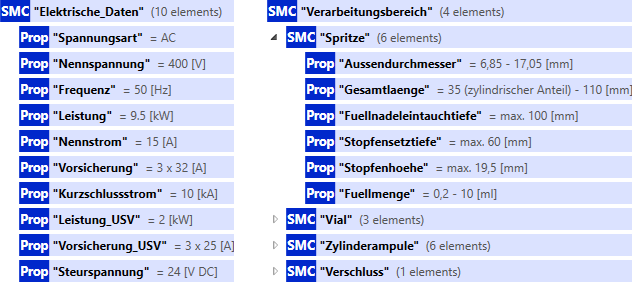
\includegraphics[width=1\textwidth]{Bilder/Ergebnisse/StatischeDaten/TechnischeDaten.png}
%     \caption{Metadatenstruktur im Submodell Dokumentation}
%     \label{fig:Doku}
% \end{figure}

% Das Submodell bildet die relevanten Maschineneigenschaften strukturiert und übersichtlich ab und übernimmt damit die Funktion der klassischen technischen Datenblätter in digitaler Form. 
% Dadurch wird eine standardisierte und leicht zugängliche Dokumentation der technischen Parameter ermöglicht.

% \subsubsection*{Dokumente und 3D-Modelle}
% \vspace{-0.5em}
% Im Submodell Dokumentation werden alle relevanten Unterlagen zur Maschine und ihren Komponenten gepflegt.
% In dieser Arbeit sind exemplarisch Dokumente wie die Betriebsanleitung, Funktionsspezifikationen, eine Netzwerkübersicht sowie die Projektzeichnung eingebunden.
% Diese sind als File-Elemente direkt in die \acs{aas}-Struktur eingebettet.

% Allerdings umfasst die Dokumentation mehr als nur das Einfügen von Dateien.
% Jedes Dokument ist in einer eigenen \acs{smc} organisiert, die dem \acs{smt} HandoverDocumentation \cite{SpezifikationDokumentation} folgt.
% Darin sind strukturierte Metadaten wie eine eindeutige Dokumentenkennung, Klassifikation und Versionsinformationen hinterlegt.
% Abbildung \ref{fig:Doku} zeigt die Metadatenstruktur am Beispiel der Funktionsspezifikationen.

% \begin{figure}[htbp]
%     \centering
%         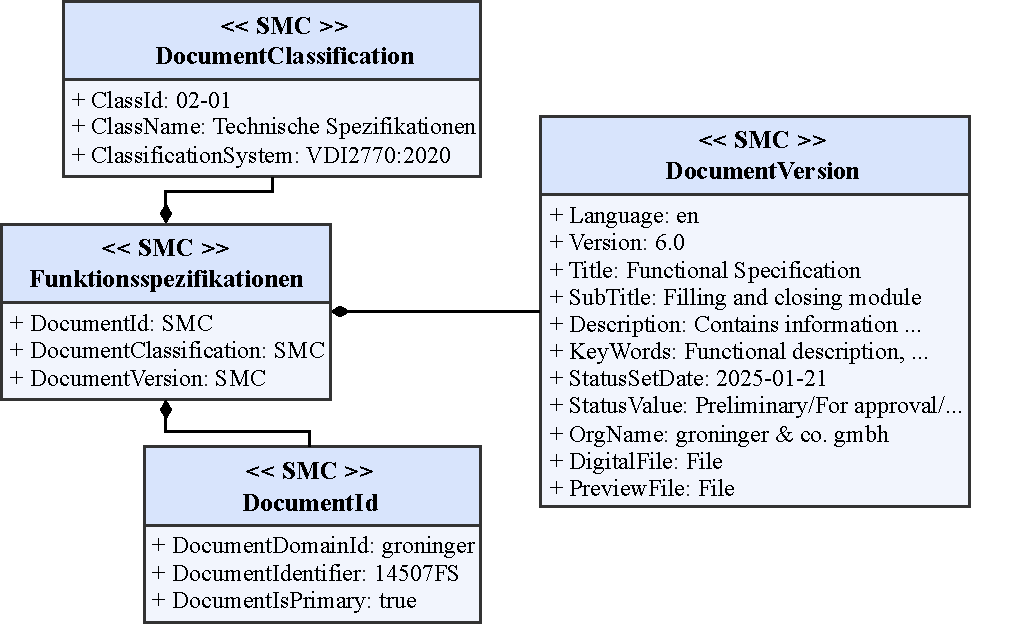
\includegraphics[width=1\textwidth]{Bilder/Ergebnisse/StatischeDaten/Doklumentation.pdf}
%     \caption{Metadatenstruktur im Submodell Dokumentation}
%     \label{fig:Doku}
% \end{figure}

% Die gezeigte Struktur ist universell einsetzbar und kann für beliebige Dokumenttypen verwendet werden, so auch für 3D-Modelle.
% Zwar existiert mit dem \acs{smt} Provision of 3D-Models \cite{Spezifikation3DModelle} ein speziell dafür vorgesehenes, deutlich umfangreicheres Template, dessen Aufbau der Dokumentationsstruktur ähnelt, jedoch zusätzliche Felder wie die geometrische Beschreibung oder Darstellungsoptionen enthält.

% In der Praxis stellt sich jedoch die Frage, ob der zusätzliche Aufwand zur vollständigen Umsetzung dieses Templates gerechtfertigt ist, insbesondere dann, wenn die dafür benötigten Daten nicht vollständig vorliegen oder nicht gepflegt werden.
% Aus diesem Grund wurde in dieser Arbeit auf eine vereinfachte Struktur zurückgegriffen, die sich an der Dokumentationslogik orientiert.

% Sowohl Dokumente als auch 3D-Modelle lassen sich über entsprechende Plugins in der AAS Web UI (Typ-2-\acs{aas}) sowie im Package Explorer (Typ-1-\acs{aas}) visualisieren und herunterladen.
% Dies ermöglicht eine einfache Nutzung und einen direkten Zugriff auf die eingebundenen Inhalte.

% \subsubsection{Hierarchische Strukturen}
% \vspace{-0.5em}

% Stücklisten spielen für Maschinenbauer eine zentrale Rolle, da sie die komplexe Zusammensetzung von Maschinen aus zahlreichen Einzelkomponenten abbilden.
% Die betrachtete robocell-Maschine besteht aus über 8.000 verschiedenen Komponenten.
% Um den Umfang überschaubar zu halten, wurde in dieser Arbeit eine Auswahl relevanter Komponenten festgelegt, die auf zwei untergeordnete Ebenen beschränkt ist.
% Jede dieser Komponenten wurde als eigenständige \acs{aas} modelliert, wodurch eine modulare und erweiterbare Struktur entsteht.

% Zur Abbildung der hierarchischen Beziehungen zwischen diesen Komponenten wurde das \acs{smt} Hierarchical Structures enabling Bills of Material \cite{SpezifikationHierachischeStrukturen} eingesetzt, das hier als \acs{bom}-Submodell bezeichnet wird.
% Nicht nur die Haupt-\acs{aas} besitzt ein solches Submodell, sondern auch jede untergeordnete Komponente.
% Dadurch lässt sich die gesamte Maschine rekursiv abbilden, indem die hierarchische Struktur in mehreren Ebenen dargestellt wird.

% Abbildung \ref{fig:BOM} zeigt diese Struktur exemplarisch.
% Im Zentrum steht das \acs{bom}-Submodell der Haupt-\acs{aas}, das die erste untergeordnete Ebene abbildet.
% Links und rechts sind referenzierte Komponenten-\acs{aas} dargestellt, die über Entity-Elemente mit der Haupt-\acs{aas} verknüpft sind und ihrerseits weitere untergeordnete Ebenen beeinhalten.

% \vspace{0.5em}
% \begin{figure}[htbp]
%     \centering
%         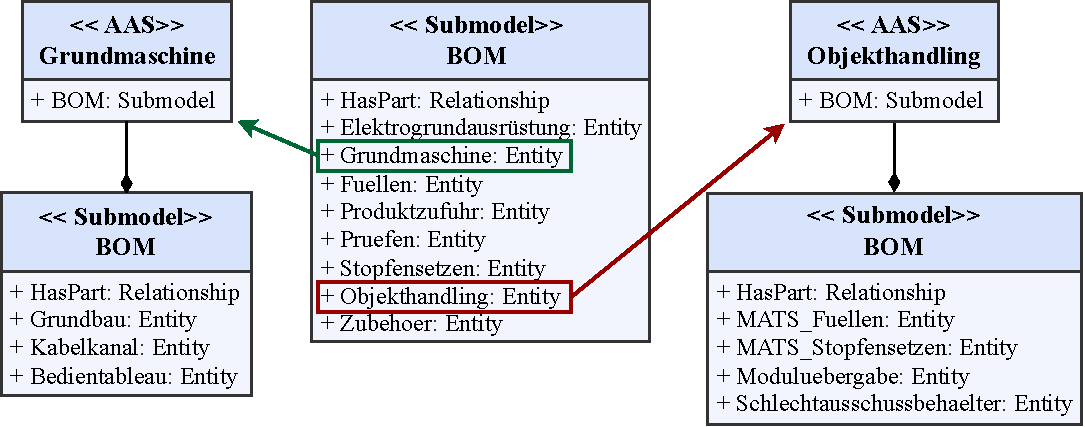
\includegraphics[width=1\textwidth]{Bilder/Ergebnisse/StatischeDaten/BOM.pdf}
%     \caption{Systemarchitektur AAS-Demonstrator}
%     \label{fig:BOM}
% \end{figure}

% Die einzelnen Komponenten sind als Self-Managed Entities modelliert, da sie jeweils über eine eigene \acs{aas} verfügen.
% Die Referenzierung erfolgt über die globalAssetId, wodurch eine direkte Verbindung zur jeweiligen Komponente hergestellt wird.
% Zur Abbildung der Beziehungen zwischen ihnen wird ein RelationshipElement verwendet.
% Primär kommt dabei die Beziehung HasPart zum Einsatz, deren Bedeutung über eine zugewiesene semanticId eindeutig definiert ist.

% Die AAS Web UI bietet ein Plugin zur Visualisierung dieser Strukturen. 
% In der grafischen Oberfläche werden die Komponenten mit ihren jeweiligen Beziehungen visuell dargestellt. 
% Abbildung \ref{fig:BOMVisualisierungUI} zeigt ein Beispiel der Grundmaschine.

% \newpage
% \begin{figure}[htbp]
%     \centering
%         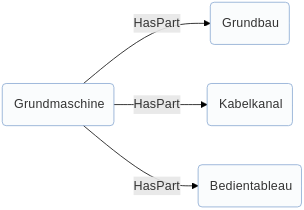
\includegraphics{Bilder/Ergebnisse/StatischeDaten/BOMVisualisierung.png}
%     \caption{BOM-Visualisierung der Grundmaschine in der AAS Web UI}
%     \label{fig:BOMVisualisierungUI}
% \end{figure}

% Wird eine Komponente innerhalb der Visualisierung selektiert, erfolgt eine direkte Navigation zur zugehörigen \acs{aas}. 
% Diese Verlinkung basiert auf der globalAssetId und setzt voraus, dass die entsprechende Komponente im Discovery Service registriert ist. 
% Dort ist für jede Komponente ein Eintrag hinterlegt, der die globalAssetId mit der eindeutigen ID der jeweiligen \acs{aas} verknüpft. 
% Die AAS Web UI nutzt diese Informationen, um die entsprechende \acs{aas} automatisch aufzulösen und in der Benutzeroberfläche anzuzeigen.

% \subsubsection{Wartungsdaten}
% \vspace{-0.5em}
% Das Submodell Wartung bildet den digitalen Wartungsplan der robocell-Maschine ab. 
% Es enthält strukturierte Informationen zu einzelnen Komponenten, darunter der letzte Wartungszeitpunkt, das Wartungsinterval, die zuständige Person oder Organisation sowie die durchzuführenden Maßnahmen. 
% Diese Informationen sind für jede Komponente in einer \acs{smc} organisiert.

% Abbildung \ref{fig:Wartung} zeigt exemplarisch die Wartungsinformationen für zwei Komponenten.

% \begin{figure}[htbp]
%     \centering
%         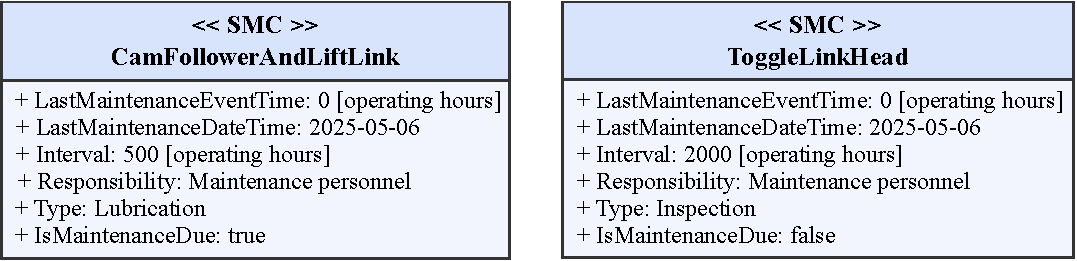
\includegraphics[width=1\textwidth]{Bilder/Ergebnisse/StatischeDaten/Wartung.pdf}
%     \caption{Systemarchitektur AAS-Demonstrator}
%     \label{fig:Wartung}
% \end{figure}

% Sofern die \acs{aas} über eine geeignete Plattform wie Eclipse BaSyx bereitgestellt wird, besteht die Möglichkeit, Wartungsmaßnahmen direkt in der AAS zu erfassen und in den Wartungsplan einzutragen. 
% Bedienpersonal sowie interne oder externe Wartungsteams könnten über entsprechende Schnittstellen oder Benutzeroberflächen Einträge vornehmen, wodurch eine nachvollziehbare Dokumentation aller Wartungsaktivitäten gewährleistet wird.

% Das Submodell wurde so entworfen, dass es künftig dynamisch erweitert werden kann. 
% Beispielsweise könnte ein Betriebsstundenzähler angebunden werden. 
% Eine entsprechende Logik oder ein Skript könnte dann den aktuellen Wert mit dem letzten Wartungszeitpunkt vergleichen und automatisch den Wartungsbedarf erkennen. 
% In jeder \acs{smc} wurde dafür eine Property implementiert, die über ein Boolean-Feld angibt, ob eine Wartung fällig ist.

% Eine weitere denkbare Optimierung besteht in der Kombination mit Predictive Maintenance.
% Der Wartungsbedarf würde dabei nicht mehr ausschließlich statisch anhand der Betriebsstunden ermittelt, sondern aktiv durch die Auswertung von Sensordaten und Analysen prognostiziert werden.
% Analog könnte dabei eine Property gesetzt werden, die nicht nur angibt, ob eine Wartung fällig ist, sondern gegebenenfalls auch die Dringlichkeit bewertet.
% Solche erweiterten Ansätze erfordern jedoch in der Regel zusätzliche Datenintegration und komplexere Algorithmen, was über den hier dargestellten Demonstrator hinausgeht.

\newpage
\subsubsection{Statische Submodelle}
Die statische Modellierung des Demonstrators erfolgte vollständig im Package Explorer.
Dazu wurden alle relevanten AAS sowie die zugehörigen Submodelle angelegt, mit Inhalten befüllt und mit einer eindeutigen ID versehen.
Als Hauptdatenquellen dienten die technischen Dokumentationen der robocell, insbesondere die Betriebsanleitung, sowie Informationen aus dem PLM-System Agile.

Abbildung~\ref{fig:PackageExplorerRobocell} zeigt die Gesamtübersicht des Abfüll- und Verschließmoduls im Package Explorer.
Die statischen Submodelle sind darin mit einer Nummer gekennzeichnet, die der im Folgenden verwendeten Gliederung entspricht.
Zur besseren Veranschaulichung seiner Funktionsweise wird das Submodell BOM ausführlicher beschrieben.
Die grundlegende Struktur der übrigen Submodelle ist im Anhang~\ref{sec:AnhangSubmodelle} anhand von Screenshots dokumentiert.

\begin{figure}[htbp]
    \centering
        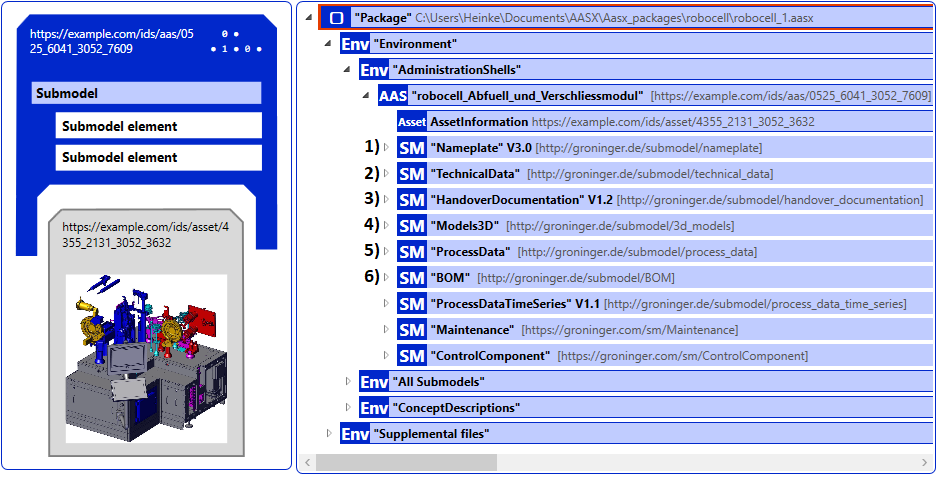
\includegraphics[width=1\textwidth]{Bilder/ErgebnissePackageExplorer/AASrobocell.PNG}
    \caption{Package Explorer: Gesamtübersicht AAS-Demonstrator}
    \label{fig:PackageExplorerRobocell}
\end{figure}

\subsubsection*{1) Typenschild}
\vspace{-0.5em}
\textbf{Funktion:}  
Das Submodell Typenschild bildet die zentrale digitale Identifikationsstelle innerhalb des Demonstrators. 
Es entspricht funktional einem physischen Typenschild, erweitert dessen Informationen jedoch um maschinenlesbare und interoperable Inhalte. 
Dadurch können die Daten nicht nur lokal angezeigt, sondern auch automatisiert in anderen Systemen verarbeitet werden.

\textbf{Inhalte:}  
Die Struktur basiert auf dem \acs{smt} Digital Nameplate for Industrial Equipment~\cite{SpezifikationTypenschild}.  
Erfasst werden grundlegende Identifikationsdaten (z.\,B. Hersteller, Seriennummer, Produkttyp) sowie erweiterte Informationen wie Softwareversionen, Zertifikate, Logos, Kontaktinformationen und weitere produktspezifische Details.

\textbf{Besonderheiten:}  
Das digitale Typenschild ermöglicht eine erweiterte Darstellung im Vergleich zu klassischen Maschinentypenschildern. In der AAS Web UI kann das Submodell als eigenes Plugin visualisiert werden. 
Die Ansicht ist dabei in zwei Bereiche gegliedert: Herstellerinformationen und Produktinformationen.

\subsubsection*{2) Technische Daten}
\vspace{-0.5em}
\textbf{Funktion:}  
Das Submodell Technische Daten dient als digitales technisches Datenblatt der Maschine.
Es ermöglicht eine standardisierte und strukturierte Abbildung aller relevanten Maschineneigenschaften und ersetzt damit die klassischen technischen Angaben aus der Betriebsanleitung.

\textbf{Inhalte:} 
Die Struktur orientiert sich am generischen SMT Technical Data~\cite{SpezifikaitonTechnischeDaten} und gliedert sich in zwei Hauptbereiche: Allgemeine Informationen und Technische Eigenschaften.
Letztere sind in mehreren \acsp{smc} organisiert, darunter Produktionsmedien, Umgebungsbedingungen, elektrische Daten sowie der Verarbeitungsbereich.
Jede \acs{smc} enthält verschiedene Elemente, überwiegend Properties oder Ranges, die einzelne Parameter, beispielsweise elektrische Kenndaten der Maschine, beschreiben.
Ein Überblick über die Struktur des Submodells ist im Anhang~\ref{subsec:TechnischeDaten} in Abbildung~\ref{fig:SMTechnischeDaten} dargestellt.

\textbf{Besonderheiten:}  
Alle zentralen technischen Informationen der Maschine sind in diesem Submodell strukturiert an einem Ort gebündelt.
Dadurch entfällt die Notwendigkeit, diese Daten in verschiedenen Systemen oder Dokumenten separat zu pflegen.

\subsubsection*{3) BOM}
\vspace{-0.5em}
\textbf{Funktion:}  
Die betrachtete robocell-Maschine besteht aus einer Vielzahl unterschiedlicher Komponenten.
Im Rahmen des Demonstrators wurde eine repräsentative Auswahl dieser Komponenten als eigenständige AAS modelliert, um die Struktur der Maschine modular abzubilden.
Das BOM-Submodell dient dazu, diese Struktur sichtbar zu machen und die Beziehungen zwischen den Komponenten hierarchisch abzubilden, vergleichbar mit einer digitalen Stückliste.

\textbf{Inhalte:}  
Die Umsetzung orientiert sich an der SMT-Spezifikation Hierarchical Structures enabling Bills of Material~\cite{SpezifikationHierachischeStrukturen}.  
Das BoM-Submodell enthält Entity-Elemente, die jeweils eine untergeordnete Komponente repräsentieren.  
Self-Managed Entities verweisen dabei über ihre globalAssetId eindeutig auf eine eigene AAS.  
Die Beziehungen zwischen den Komponenten werden über Relationship-Elemente mit einer eindeutigen semanticId gemäß der SMT-Spezifikation beschrieben.  

Zur Veranschaulichung wurde das Bedientableau als Beispiel gewählt, da es weniger komplex als die Maschinenebene ist, aber dennoch alle relevanten Strukturelemente enthält.  
Abbildung~\ref{fig:BOMSubmodelGrundmashcine} zeigt das BoM-Submodell der Grundmaschine, in dem das Bedientableau als Self-Managed Entity aufgeführt ist.  
Über die globalAssetId ist es mit seiner eigenen AAS verknüpft (Abbildung~\ref{fig:AASBedientableau}), die wiederum ein eigenes BoM-Submodell mit weiteren Unterkomponenten enthält.  
Dieses Beispiel verdeutlicht die rekursive Struktur, mit der sich die gesamte Maschine in beliebig viele Hierarchieebenen gliedern lässt.

\begin{figure}[htbp]
    \centering
        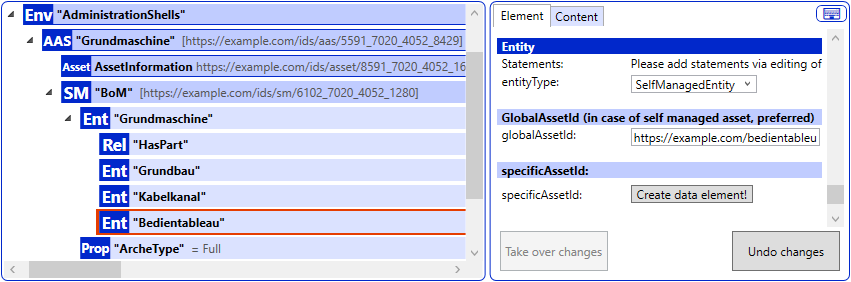
\includegraphics[width=1\textwidth]{Bilder/ErgebnissePackageExplorer/GundmaschneEntitie.PNG}
    \caption{Package Explorer: BOM-Submodell der Grundmaschine}
    \label{fig:BOMSubmodelGrundmashcine}
\end{figure}

\begin{figure}[htbp]
    \centering
        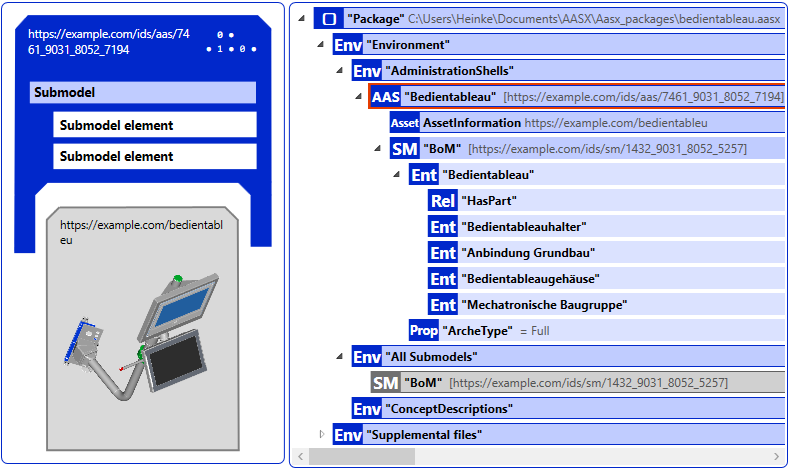
\includegraphics[width=1\textwidth]{Bilder/ErgebnissePackageExplorer/Bedientableau+.PNG}
    \caption{Package Explorer: AAS des Bedientableaus}
    \label{fig:AASBedientableau}
\end{figure}

\textbf{Besonderheiten:}  
Das BOM-Submodell ermöglicht eine modulare Modellierung, bei der jede Komponente als eigenständiges Asset mit eigener AAS geführt wird.  
Dadurch bleibt die Struktur flexibel erweiterbar und unabhängig von der Hauptkomponente.  
Falls die globalAssetId einer Komponente nicht bekannt ist, kann diese über den Discovery Service in Eclipse BaSyx ermittelt werden, was eine dynamische Suche und Verknüpfung von AAS im Gesamtsystem ermöglicht.

\subsubsection*{4), 5) Dokumentation und 3D-Modelle}
\vspace{-0.5em}
\textbf{Funktion:}  
Die Submodelle Dokumentation und 3D-Modelle dienen der strukturierten Bereitstellung und semantischen Klassifizierung von digitalen Dateien.  
Während das Submodell Dokumentation allgemeine technische Unterlagen wie Betriebsanleitungen oder Zeichnungen verwaltet, umfasst das Submodell 3D-Modelle digitale Geometriedaten, die den Aufbau der Maschine und ihrer Komponenten beschreiben. 

\textbf{Inhalte:}  
Die Struktur des Submodells Dokumentation basiert auf dem SMT Handover Documentation~\cite{SpezifikationDokumentation}.  
Es enthält technische Unterlagen wie beispielsweise die Netzwerkübersicht oder die Projektzeichnung des Abfüll- und Verschließmoduls.  
Diese sind als File-Elemente direkt in die AAS eingebettet und jeweils in einer eigenen \acs{smc} organisiert.  
Jede smc enthält zentrale Metainformationen wie Identifikation, Klassifikation und Versionsinformationen, wodurch die Dokumente eindeutig beschrieben und rückverfolgbar sind.  
Die vollständige Struktur einer solchen \acs{smc} ist exemplarisch im Anhang in Abbildung~\ref{fig:SMDokumentation} am Beispiel Funktionsspezifikationen dargestellt.

Das Submodell 3D-Modelle orientiert sich am SMT Provision of 3D-Models~\cite{Spezifikation3DModelle}, wurde im Demonstrator jedoch in vereinfachter Form umgesetzt.  
Die Geometriedaten umfassen Konstruktionsdateien in Form von CAD-Modellen und sind analog zum Submodell Dokumentation eingebettet und beschrieben.  
Eine Erweiterung um zusätzliche Metadaten, wie Darstellungsoptionen oder Geometrieinformationen, wäre möglich, wurde im Demonstrator jedoch nicht umgesetzt.  

\textbf{Besonderheiten:}  
Beide Submodelle sind universell einsetzbar und können flexibel um zusätzliche Dokumente oder Modelle erweitert werden.  
Die eindeutige Beschreibung der Inhalte gemäß SMT-Spezifikation stellt sicher, dass sie sowohl von Menschen als auch von technischen Systemen interpretiert und über den gesamten Lebenszyklus hinweg rückverfolgt werden können.  
In der AAS Web UI sowie im Package Explorer stehen zudem spezielle Plugins zur Verfügung, über die die Inhalte direkt angezeigt oder die hinterlegten Dateien heruntergeladen werden können, wodurch ein schneller Zugriff und eine einfache Weiterverwendung ermöglicht wird.

\subsubsection*{6) Wartung}
\vspace{-0.5em}
\textbf{Funktion:}  
Das Submodell Wartung bildet den digitalen Wartungsplan der Maschine ab.  
Es ermöglicht die strukturierte Verwaltung von Wartungsinformationen innerhalb des Demonstrators und gewährleistet dadurch eine nachvollziehbare Dokumentation, beispielsweise für Wartungspersonal.

\textbf{Inhalte:}  
Für jede Komponente werden letzte Wartungszeitpunkte, Wartungsintervalle, zuständige Personen oder Organisationen sowie durchzuführende Maßnahmen in eigenen \acs{smc} erfasst.  
Diese Struktur erlaubt eine gezielte und übersichtliche Dokumentation aller Wartungsaktivitäten.

\textbf{Besonderheiten:}  
Das Submodell ist so konzipiert, dass es zukünftig dynamisch erweitert werden kann, beispielsweise durch die Anbindung eines Betriebsstundenzählers, der Wartungsbedarf automatisch erkennen kann.  
Ebenso ist die Integration von Predictive-Maintenance-Ansätzen denkbar, um Wartungsbedarf vorausschauend anhand von Sensordaten zu ermitteln.

% \textbf{Zusammenfassung}  
% Die Stammdaten der Maschine zentral an einem Ort
% Darin alle standardisiert beschriben mit enideutiger Semantik beschreiben mit Concept Descripotions, dadurch auch maschinenverständlich
% Was ist jetzt der Vorteil davon. Die Daten können alle ganz einfach als Typ-1-AAS im AASX Datei Format an Interessenten weitergegeben werden
% Diese Könnten die dann einfach an die bestehenden Unternehmenssystem angebunden und autimatisch im ERP oder PLM die Datenn gemappt, sofern eine geeignet Struktur vorhanden also hier will ich sagen das die aas quasi der robocell weitergegebn werden kann
% Genauso aber auch umgekehrt, wie mit der hierachischen Abbildung gezeigt so auch bei groninger hier dann umgekehrt für groninger auch, weil interessant für Maschinenabuer und nicht nur für die System sondern auch direkt in den die AAS der Maschine eingebettet

\newpage
\subsubsection{Dynamische Submodelle}
\label{sec:DynamischeSubmodelle}
Neben den statischen Submodellen wurden im Demonstrator auch dynamische Submodelle umgesetzt.
Sie ermöglichen die kontinuierliche Erfassung und Aktualisierung von Maschinen- und Prozessdaten sowie die Interaktion mit dem zugrunde liegenden Asset.
Da im Rahmen dieser Arbeit keine reale Maschine zur Verfügung stand, wird dieses Asset durch den Datengenerator und den Maschinensimulator repräsentiert.

Die technische Umsetzung und die zugrunde liegenden Datenflüsse orientieren sich an etablierten Industriearchitekturen, sodass die Schnittstellen und Funktionsweisen ohne Anpassungen auch mit einem realen System genutzt werden könnten.
Durch diese Erweiterung erfüllt der Demonstrator die Anforderungen an einen digitalen Zwilling gemäß der in Kapitel~\ref{sec: DT} beschriebenen Klassifizierung.

\subsubsection*{Prozessdaten}

Das Submodell Prozessdaten dient der Erfassung und Bereitstellung zentraler Betriebsinformationen.
Im Rahmen dieser Arbeit wurden exemplarisch die Messgrößen Füllstand, Durchfluss, Anzahl abgefüllter Einheiten und Druck implementiert.
Die Werte stammen aus dem \acs{opcua}-Server des Datengenerators, der sie im Sekundentakt aktualisiert und über die Databridge nahezu in Echtzeit an die \acs{aas} überträgt.
Vor der Speicherung im Submodel Repository erfolgt eine zweistufige Transformation.
Zunächst werden die Rohdaten mithilfe des Jackson-Transformers in ein JSON-Format überführt, anschließend extrahiert JSONata die relevanten Messgrößen, die schließlich den entsprechenden Properties des Submodells zugeordnet werden.

Die Visualisierung der Prozessdaten erfolgt in der klassischen Elemente-Ansicht der AAS Web UI, wie in Abbildung~\ref{fig:Processdata} dargestellt, oder über ein speziell entwickeltes Plugin.
Damit die Werte in der Benutzeroberfläche aktuell bleiben, kann eine Synchronisationsfunktion aktiviert werden.
Dabei ruft die Weboberfläche die relevanten Daten in festen Intervallen, beispielsweise alle vier Sekunden, automatisch vom Repository ab.

\newpage
\begin{figure}[htbp]
    \centering
    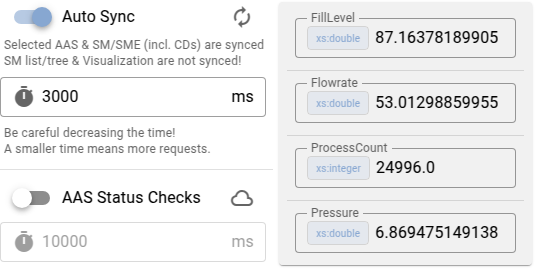
\includegraphics[width=1\textwidth]{Bilder/Ergebnisse/DynamischeDaten/ProcessData/VisualisierungNeu.png}
    \caption{AAS Web UI: Prozessdaten}
    \label{fig:Processdata}
\end{figure}

Die Umsetzung ist protokolloffen und könnte grundsätzlich auf weitere Kommunikationsstandards wie \acs{mqtt} oder \acs{rest} erweitert werden.
Eine automatische bidirektionale Kommunikation, etwa das Zurückschreiben von Werten aus der \acs{aas} in externe Systeme, ist mit der eingesetzten Databridge derzeit jedoch nicht möglich.

\subsubsection*{Kontrollkomponente}
Das Submodell Kontrollkomponente dient der Abbildung und Visualisierung des aktuellen Maschinenstatus sowie der unterstützten Betriebsmodi.
Die Zustandsinformationen stammen aus dem Maschinensimulator, der sie in numerischer Form über einen \acs{opcua}-Server bereitstellt.
Über die Databridge werden diese Werte in nahezu Echtzeit in die \acs{aas} übertragen.
Vor der Speicherung erfolgt eine semantische Umwandlung mithilfe von JSONata, um die numerischen Codes in sprechende Zustandsbezeichnungen zu überführen.

Die Zustände orientieren sich am PackML-Standard (Packaging Machine Language), einem von der OMAC (Organization for Machine Automation and Control) entwickelten Modell zur einheitlichen Beschreibung von Maschinenzuständen und zulässigen Zustandsübergängen, insbesondere für Verpackungsmaschinen \cite{OMAC}. 
Der Standard definiert insgesamt 17 Maschinenzustände und legt fest, welche Übergänge zwischen diesen möglich sind. 
Dieses Konzept kommt auch bei der robocell-Linie zum Einsatz und ermöglicht eine konsistente und interoperable Erfassung des Maschinenstatus über verschiedene Systeme hinweg.

Die Visualisierung erfolgt über ein in die AAS Web UI integriertes Vue.js-Plugin, das den Maschinenstatus als PackML-Zustandsautomat darstellt.
Das Plugin basiert auf einer Entwicklung der Hochschule für Technik und Wirtschaft Berlin \cite{HTW1, HTW2} und wurde funktional angepasst, um es in die AAS Web UI zu integrieren und die im Demonstrator benötigten Steuer- und Anzeigeoptionen zu unterstützen.
Abbildung~\ref{fig:PackMLZustandsautomat} zeigt die Darstellung des PackML-Zustandsautomaten in der Benutzeroberfläche.
Damit Statusänderungen unmittelbar sichtbar werden, ist eine Polling-Logik implementiert, die den aktuellen Maschinenstatus in festen Intervallen aus dem Submodel Repository der AAS Environment abruft und im Zustandsautomaten aktualisiert.

\begin{figure}[htbp]
    \centering 
    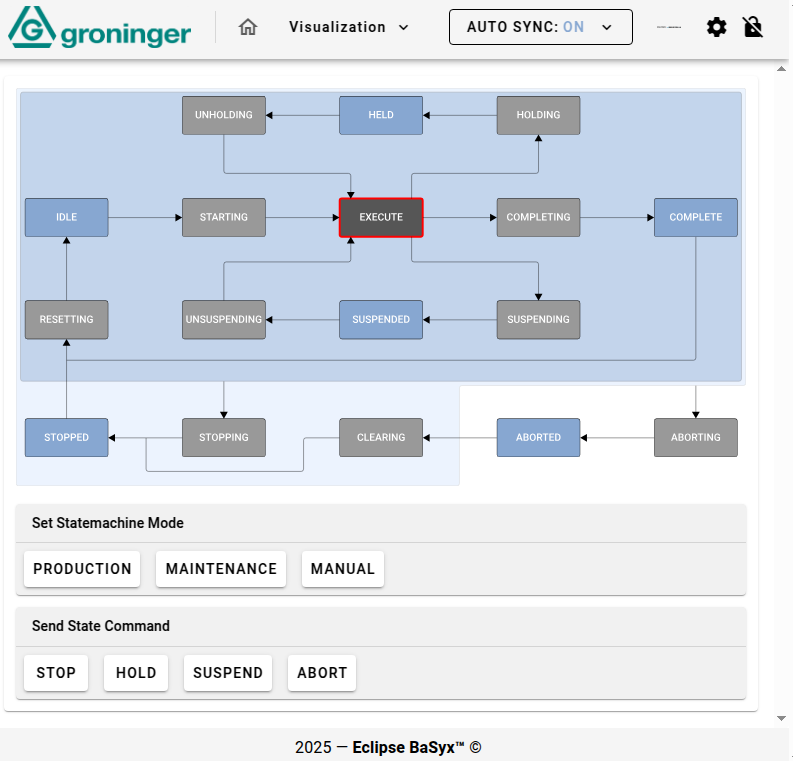
\includegraphics[width=1\textwidth]{Bilder/Ergebnisse/DynamischeDaten/Kontrollkomponente/Visualisierung.png} 
    \caption{AAS Web UI: PackML-Zustandsautomat} 
    \label{fig:PackMLZustandsautomat} 
\end{figure}

Neben der reinen Statusanzeige erlaubt das Plugin auch die Steuerung zulässiger Zustandsübergänge direkt aus der Benutzeroberfläche heraus.
Befindet sich die Maschine beispielsweise im Zustand Execute, können Befehle wie Stop, Hold, Suspend oder Abort ausgelöst werden.
Darüber hinaus lässt sich der Betriebsmodus (Produktion, Manuell oder Wartung) setzen, der ebenfalls als Property im Submodell verwaltet wird.

Im Demonstrator werden Befehle direkt per WebSocket an den Maschinensimulator übermittelt und dort ohne weitere Prüfungen übernommen. 
Dadurch entsteht eine direkte Feedback-Schleife zwischen der \acs{aas} und dem simulierten Asset.
In einer realen Maschine würden diese Signale hingegen zunächst über ein geeignetes Industrieprotokoll wie \acs{opcua} an die speicherprogrammierbare Steuerung (SPS) übertragen und dort validiert werden müssen, bevor der neue Zustand an die \acs{aas} zurückgemeldet wird.

\subsubsection*{Zeitreihendaten}
Das Submodell Zeitreihendaten dient der Einbettung historischer Messwerte in die \acs{aas}. 
Im Demonstrator werden hierfür exemplarisch die Messgrößen Druck und Temperatur verwendet, die kontinuierlich vom \acs{opcua}-Server des Datengenerators bereitgestellt werden. 
Anstatt diese Werte direkt in der \acs{aas} abzulegen, werden sie mithilfe von Telegraf in eine externe InfluxDB-Datenbank übertragen. 
Telegraf abonniert dazu die relevanten Variablen des \acs{opcua}-Servers und schreibt geänderte Werte unmittelbar in die Datenbank.

Die Anbindung an die \acs{aas} erfolgt über ein LinkedSegment (eine \acs{smc}) im Submodell, das alle für die Datenabfrage erforderlichen Parameter enthält, wie den Endpunkt der InfluxDB und die zugehörige Abfragebeschreibung. 
Dadurch können Anwendungen, die auf die \acs{aas} zugreifen, die Zeitreihendaten gezielt abrufen, ohne Details zur technischen Implementierung der Datenbank kennen zu müssen.

Zur Visualisierung steht in der AAS Web UI ein spezielles Plugin zur Verfügung, das auf die im LinkedSegment hinterlegten Parametern zugreift und Abfragen an die InfluxDB stellt. 
Ein Nutzer kann dabei auswählen, ob einzelne Messgrößen oder kombinierte Ansichten mehrerer Werte angezeigt werden sollen. 
Abbildung~\ref{fig:LiniendiagrammBaSyx} zeigt exemplarisch ein Liniendiagramm mit den zeitlichen Verläufen von Druck und Temperatur über einen Zeitraum von fünf Minuten.

\begin{figure}[htbp]
    \centering
        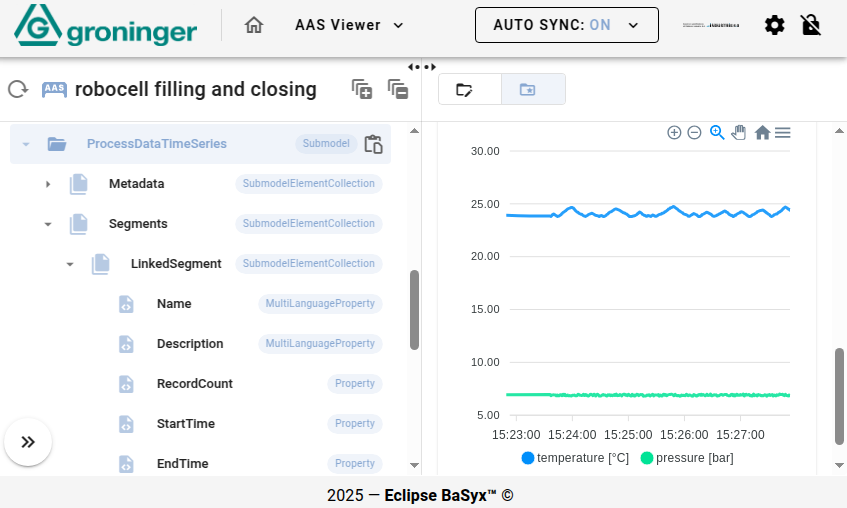
\includegraphics[width=1\textwidth]{Bilder/Ergebnisse/DynamischeDaten/ZeitreihenDaten/Liniendiagramm.png}
    \caption{AAS Web UI: Zeitreihendaten (Liniendiagramm)}
    \label{fig:LiniendiagrammBaSyx}
\end{figure}

Ein wesentlicher Vorteil dieser Umsetzung liegt in der Entkopplung von Datenspeicherung und \acs{aas}. 
Da die \acs{aas} selbst nicht für die Ablage großer oder historischer Datenmengen ausgelegt ist, ermöglicht die Auslagerung in eine externe Zeitreihendatenbank eine effiziente Speicherung und Verarbeitung. 
Zudem können die Daten durch die strukturierte Referenzierung über das LinkedSegment einfach in weiteren Anwendungen, wie Analysesystemen oder KI-gestützten Verfahren, weiterverwendet werden.

\newpage
\subsubsection{Herausforderungen bei der Implementierung}
Im Rahmen der Implementierung des Demonstrators traten verschiedene Herausforderungen auf, die sowohl technische als auch methodische Aspekte betrafen. 
Diese ergaben sich unter anderem aus der noch jungen Verbreitung der \acs{aas} im Maschinenbau, der eingeschränkten Datenverfügbarkeit sowie den Limitierungen der eingesetzten Werkzeuge. 
Die wesentlichen Punkte sind im Folgenden zusammengefasst:

\begin{enumerate}
    \item \textbf{Fehlende praxisnahe Vorlagen für den Maschinenbau:}  
    Zwar existieren bereits diverse \acsp{smt}, Spezifikationen sowie allgemeine Anwendungsfälle, diese sind jedoch primär auf Komponentenhersteller ausgerichtet.  
    Konkrete Vorlagen und praxisnahe Anwendungsfälle, die speziell auf den Maschinenbau und die Anforderungen des Demonstrators zugeschnitten sind, standen jedoch nur begrenzt zur Verfügung.

    \item \textbf{Begrenzte Datenverfügbarkeit:}  
    Da keine reale Maschine angebunden war, mussten Echtzeitdaten simuliert werden.  
    Zudem waren nicht alle relevanten Daten im PLM-System so dokumentiert, dass eine direkte Übernahme möglich gewesen wäre.  
    Viele Informationen mussten daher manuell aus verschiedenen Dokumenten, wie der Betriebsanleitung, extrahiert werden.  

    \item \textbf{Begrenzte Verfügbarkeit semantischer Beschreibungen:}  
    Für viele spezifische Maschineneigenschaften, wie technische Parameter im Verarbeitungsbereich (z.\,B. Spritze, Vial, Zylinderampulle) und deren Detailwerte (z.\,B. Füllmenge, Stopfenhöhe), existieren bislang keine standardisierten ECLASS-Beschreibungen.  
    Diese mussten daher manuell angelegt werden, was zeitaufwendig war und die Interoperabilität einschränkt.

    \item \textbf{Eingeschränkte Funktionalität der eingesetzten Tools:}  
    Die verwendeten Werkzeuge unterstützten nicht alle benötigten Funktionen.  
    So wurden beispielsweise beim Hochladen von Dateien in der AAS Web UI keine Einträge im Discovery Service erzeugt.  
    Da diese Funktionalität erforderlich war, musste sie mithilfe eines eigens entwickelten Skripts ergänzt werden.  
    Eine detaillierte Evaluierung der eingesetzten Tools erfolgt in Kapitel~XY.

    \item \textbf{Inkonsistenzen zwischen Spezifikationen und Tools:}  
    \acsp{smt} und die zugehörigen Spezifikationen wiesen teilweise Inkonsistenzen auf, etwa unterschiedliche Werte in der Dokumentation im Vergleich zu den AASX-Vorlagen.  
    Dies führte dazu, dass einige Plugins nicht oder nur eingeschränkt funktionierten, da sie auf korrekte semantische Beschreibungen angewiesen sind.  
    Die Fehlerbehebung erforderte eine manuelle Anpassung der \acsp{smt}, was zusätzlichen Aufwand verursachte.
\end{enumerate}

%KI-Modell
\newpage
\subsection{KI-Modell zur Anomalieerkennung}

Für die Anomalieerkennung wurde der zuvor trainierte Autoencoder im Evaluierungsmodus eingesetzt, sodass während der Auswertung keine Anpassungen der Modellparameter erfolgen.
Die Testdaten basieren, wie beim Training, auf simulierten Temperaturverläufen aus dem Datengenerator, die analog zu den Zeitreihendaten in Kapitel \ref{sec:DynamischeSubmodelle} in einer InfluxDB gespeichert wurden.

Als Eingabe erhält das Modell kurze Sequenzen von jeweils fünf Messwerten.
Im Unterschied zur Trainingsphase enthalten die Testdaten gezielt eingefügte Anomalien, um die Erkennungsfähigkeit des Modells zu prüfen.
Dabei wurden vier Anomalietypen simuliert: dauerhaft erhöhte Werte, ein einzelner ausgeprägter Peak, ein linearer Anstieg über mehrere Zeitpunkte sowie invertierte Werte im Vergleich zum Normalverlauf.

Während der Auswertung berechnet der Autoencoder für jede Sequenz den Rekonstruktionsfehler als durchschnittliche Abweichung zwischen Eingabe- und Ausgabedaten. 
Zur Klassifikation dient ein Schwellenwert, der aus dem Mittelwert des Fehlers plus dem Zweifachen der Standardabweichung gebildet wird. 
Überschreitet der Fehler einer Sequenz diesen Wert, wird das gesamte Zeitfenster als Anomalie markiert.

Zur Veranschaulichung werden zwei Beispiele gezeigt, die unterschiedliche Anomalietypen repräsentieren. 
Abbildung~\ref{fig:Fall1} zeigt einen Temperaturverlauf mit dauerhaft erhöhten Werten im Bereich t = 10000 - 10010 (gezielt eingefügte Anomalie). 
Das Modell erkennt die Anomalie zuverlässig, allerdings leicht verzögert. 
Dies liegt an der Mittelwertbildung über das Fünf-Werte-Fenster.
Erst wenn mehrere aufeinanderfolgende Werte vom Normalverlauf abweichen, steigt der Fehler ausreichend an.

\begin{figure}[htbp]
    \centering
        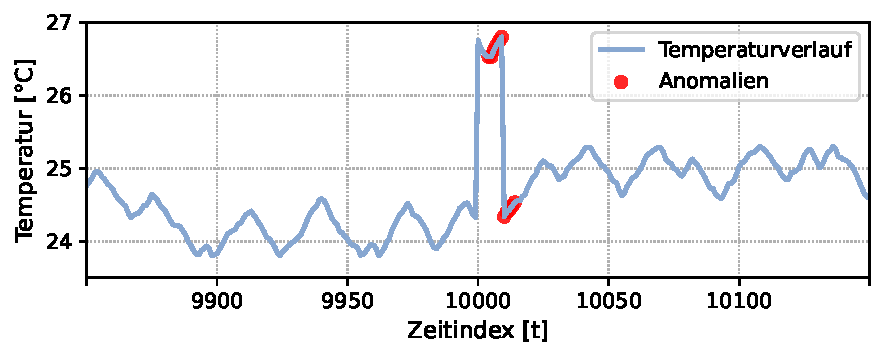
\includegraphics[width=1\textwidth]{Bilder/Ergebnisse/KI/Fall1.pdf}
        \vspace{-2em}
    \caption{Anomalieerkennung Fall 1: Überhöhte Daten}
    \label{fig:Fall1}
\end{figure}

In Abbildung~\ref{fig:Fall2} ist ein Temperaturverlauf mit einem gleichmäßigen, linearen Anstieg im Bereich t = 25343 - 25393 (gezielt eingefügte Anomalie) dargestellt. 
Auch hier klassifiziert das Modell den Verlauf korrekt als Anomalie. 
Dies zeigt, dass die Erkennung nicht nur auf plötzliche Ausreißer reagiert, sondern auch schleichende Veränderungen im Signalverlauf erkennt.


\begin{figure}[htbp]
    \centering
        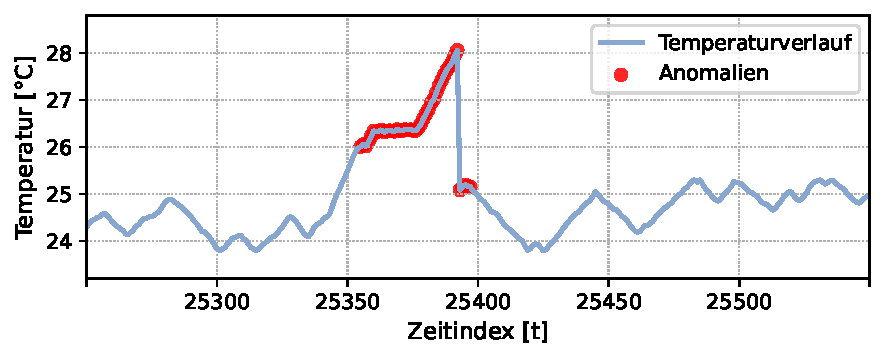
\includegraphics[width=1\textwidth]{Bilder/Ergebnisse/KI/Fall2.pdf}
        \vspace{-2em}
    \caption{Anomalieerkennung Fall 2: Linearer Anstieg}
    
    \label{fig:Fall2}
\end{figure}

In allen Testfällen mit künstlich erzeugten Anomalien erfolgte die Klassifikation korrekt, ohne Fehlalarme. 
Aufgrund der Fenstergröße und der Mittelwertbildung tritt die Markierung jedoch häufig leicht verzögert auf, wodurch einzelne Sequenzen innerhalb einer Anomaliephase nicht als abweichend markiert werden. 
Da ausschließlich synthetische Abweichungen geprüft wurden, ist zu erwarten, dass reale Anomalien aufgrund ihrer höheren Komplexität eine größere Herausforderung darstellen.

Zur Verbesserung könnten umfangreichere und variantenreichere Trainings- und Testdaten eingesetzt werden. 
Auch leistungsfähigere Architekturen wie tiefere Autoencoder oder LSTM-basierte Netze (Long Short-Term Memory, eine spezielle Form rekurrenter neuronaler Netze zur Verarbeitung von Zeitreihen) bieten Potenzial, zeitliche Abhängigkeiten präziser zu erfassen.
Diese Ansätze wurden aufgrund begrenzter Rechenressourcen im Rahmen dieser Arbeit nicht weiterverfolgt, können aber eine Grundlage für zukünftige Entwicklungen bilden.

% Digitaler Produktpass
\newpage
\subsection{Anwendungsfall Digitaler Produktpass}
Im Rahmen dieses Anwendungsfalls wird gezeigt, wie PCF-Werte für verschiedene Lebenszyklusphasen dynamisch ermittelt, aggregiert und in ein Submodell geschrieben werden. 
Grundlage bildet der in Kapitel \ref{xy} vorgestellte AAS-Demonstrator, der zu diesem Zweck um ein Submodell zur Abbildung des \acs{cf} erweitert wurde.
Anschließend wird erläutert, wie der Zugriff auf die im DPP enthaltenen Informationen geregelt ist und wie unterschiedliche Nutzergruppen sowie technische Clients auf die Inhalte zugreifen können.

\subsubsection{Abbildung des PCF}
Das \acs{cf}-Submodell enthält drei \acsp{smc}, die die Lebenszyklusphasen Material, Produktion und Cradle to Gate abbilden.
Zusätzlich ist eine Komponentenliste integriert, über die die relevanten Steuerungselemente referenziert sind.
Abbildung \ref{fig:SubmodellCF} zeigt einen Ausschnitt dieses Submodells.
Zu erkennen ist die \acs{smc} für die Phase Cradle to Gate sowie die Komponentenliste mit ausgewählten Siemens-Komponenten.

\begin{figure}[htbp]
    \centering
        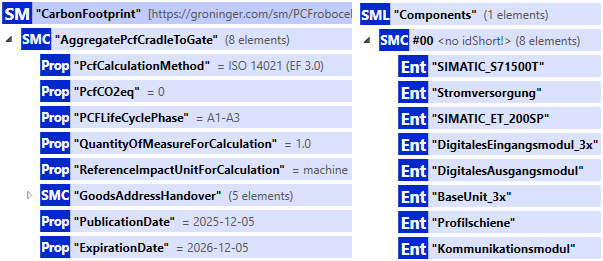
\includegraphics[width=1\textwidth]{Bilder/Ergebnisse/DPP/SubmodellCF.png}
    \caption{CF-Submodell der robocell}
    \label{fig:SubmodellCF}
\end{figure}

Die dynamische Berechnung der Gesamt-\acs{pcf}-Werte der einzelnen Phasen kann über die AAS Web UI ausgelöst werden.
Im Visualisierungsbereich wurde hierzu eine Schaltfläche implementiert, die die Aggregation der CO\textsubscript{2}-Äquivalente auslöst. 
Dies erfolgt durch das Senden einer \acs{http}-GET-Anfrage an den Microservice, der die Berechnung ausführt.

Der Microservice, der als Docker-Container implementiert wurde, reagiert auf die Anfrage und startet den Berechnungsprozess. 
Dabei nutzt er die \acs{rest}-Schnittstelle des Submodel Repositories der AAS Environment, um zunächst alle in der Komponentenliste hinterlegten Entitäten auszulesen. 
Mithilfe des Discovery Service werden auf Basis ihrer globalAssetIds die zugehörigen Komponenten-\acs{aas} identifiziert und anschließend vom AAS Repository abgerufen.

Für jede dieser Komponenten wird geprüft, ob ein \acs{cf}-Submodell vorhanden ist. 
Falls dies zutrifft, wird das Submodell ausgelesen und die darin enthaltenen \acs{pcf}-Werte extrahiert. 
Aus den ermittelten Einzelwerten berechnet der Microservice anschließend die aggregierten CO\textsubscript{2}-Äquivalente für die Phasen Produktion, Material sowie Cradle to Gate. 
Die berechneten Werte werden über die \acs{rest}-\acs{api} in das \acs{cf}-Submodell der Haupt-\acs{aas} geschrieben und stehen dort strukturiert zur Verfügung.

Außerdem sendet der Microservice eine Bestätigung an das Plugin zurück. 
Dieses reagiert darauf, indem es das aktualisierte \acs{cf}-Submodell über die \acs{rest}-Schnittstelle des Submodel Repositories abfragt. 
Die relevanten Submodellelemente werden dabei herausgefiltert und in der Benutzeroberfläche aktualisiert. 
Dadurch werden die aggregierten \acs{pcf}-Werte unmittelbar sichtbar, ohne dass ein manuelles Neuladen erforderlich ist.

Abbildung \ref{fig:PluginAggregation} zeigt die entsprechende Visualisierung. 
Auf der linken Seite sind die berechneten CO\textsubscript{2}-Äquivalente dargestellt, auf der rechten Seite die zugehörigen Lebenszyklusphasen.

\begin{figure}[htbp]
    \centering
        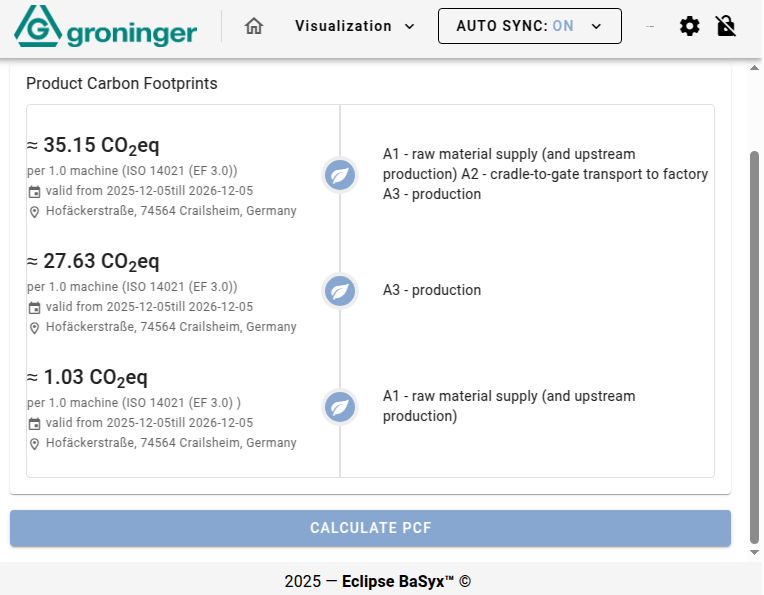
\includegraphics[width=1\textwidth]{Bilder/Ergebnisse/DPP/PluginTest.png}
    \caption{Visualisierung der aggregierten PCF-Werte}
    \label{fig:PluginAggregation}
\end{figure}

Die beschriebene Lösung ermöglicht es, den \acs{pcf} dynamisch auf Basis der in der Komponentenliste referenzierten Steuerungselemente zu berechnen. 
Auch wenn derzeit nur acht Siemens-Komponenten berücksichtigt werden, lässt sich die Liste bei Verfügbarkeit weiterer Komponenten-\acs{aas} unkompliziert erweitern, sodass sukzessive die gesamte Maschine in die Berechnung einbezogen werden kann.

Perspektivisch lässt sich die Berechnung zudem um weitere Lebenszyklusphasen wie Nutzung oder Entsorgung ergänzen, um eine ganzheitliche Betrachtung von der Herstellung bis zum Lebensende eines Produkts bzw. einer Maschine zu ermöglichen.
Darüber hinaus könnte auch der \acs{tcf} berücksichtigt werden, beispielsweise im Rahmen der Auslieferung einer Maschine, wodurch eine noch umfassendere Bilanzierung der Umweltauswirkungen ermöglicht wird.

\subsubsection{Rollenbasierter Zugriff auf Submodelle}
Der \acs{dpp} wird in diesem Anwendungsfall durch den erweiterten AAS-Demonstrator repräsentiert.  
Um sicherzustellen, dass nur autorisierte Nutzer auf spezifische Submodelle des \acs{dpp} zugreifen können, wurde eine rollenbasierte Zugriffskontrolle implementiert.  
Die Authentifizierung und Autorisierung erfolgen über Eclipse BaSyx in Kombination mit Keycloak.

Eine Möglichkeit zur Einsicht der im \acs{dpp} enthaltenen Informationen bietet die AAS Web UI.  
Ist \acs{rbac} aktiviert, wird der Benutzer beim Aufruf der Oberfläche automatisch zur Keycloak-Anmeldeseite weitergeleitet.  
Wie in Abbildung~\ref{fig:KeycloakAnmeldeSeite} dargestellt, erfolgt die Authentifizierung über die in Keycloak hinterlegten Zugangsdaten.

\begin{figure}[htbp]
    \centering
        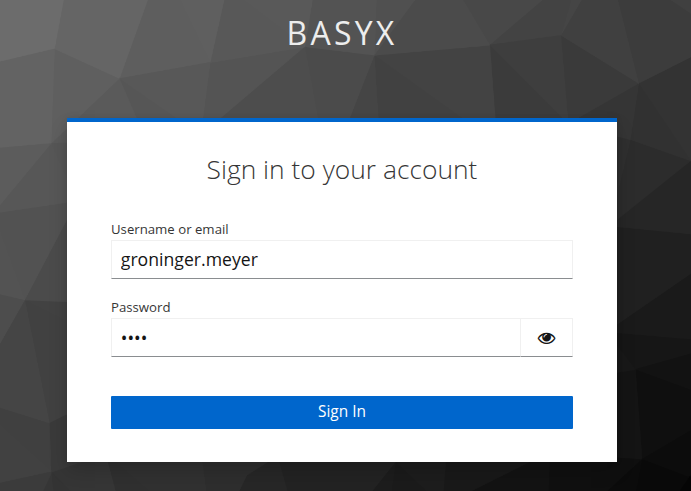
\includegraphics[width=0.7\textwidth]{Bilder/Ergebnisse/DPP/KeycloakAnmeldeSeite.png}
    \caption{Keycloak-Anmeldeseite für die AAS Web UI}
    \label{fig:KeycloakAnmeldeSeite}
\end{figure}

Nach erfolgreicher Anmeldung erhält die AAS Web UI ein Zugriffstoken, das die Rolleninformationen des Nutzers enthält.  
Dieses Token wird im Hintergrund an die angebundenen BaSyx-Komponenten weitergegeben.  
Die Entscheidung über die tatsächliche Zugriffsberechtigung trifft nicht die Web UI selbst, sondern der jeweilige Service, indem er die im Token enthaltenen Rollen gegen die hinterlegten \acs{rbac}-Regeln prüft.  
Liegt keine entsprechende Konfiguration vor, wird der Zugriff verweigert.

Meldet sich beispielsweise der Nutzer customer.doe an, so erhält er Zugriff auf den \acs{dpp}, jedoch sieht er ausschließlich jene Submodelle, die für seine Rolle freigegeben sind, etwa das Typenschild, technische Daten oder der \acs{cf}.  
Andere Submodelle wie 3D-Modelle oder Wartungsinformationen bleiben verborgen.  
Zudem besitzt der Benutzer lediglich Leserechte.
Veruscht er Änderungen an den Inhalten des \acs{dpp} vorzunehmen, so wird dies mit einem Fehler abgelehnt.

Neben dem Zugriff über die AAS Web UI ist auch ein direkter Zugriff auf die BaSyx-Komponenten über die \acs{api} möglich. 
Dies ist insbesondere für technische Clients oder externe Anwendungen relevant, die automatisiert auf die im \acs{dpp} enthaltenen Informationen zugreifen möchten.

Für diesen Anwendungsfall wurden in Keycloak drei Clients eingerichtet, denen jeweils ein Service Account zugewiesen ist. 
Diese Clients sind den Rollen Groninger-Mitarbeiter, Service-Techniker und Kunde zugeordnet und erhalten dadurch dieselben Zugriffsrechte wie die entsprechenden Benutzerkonten. 

Zur Validierung der Zugriffskonfiguration wurde das Tool Postman verwendet. 
Die Zugriffstokens wurden über den Token-Endpunkt des Realms mithilfe der Client-Anmeldedaten abgerufen und für die API-Aufrufe verwendet.

\begin{figure}[htbp]
    \centering
        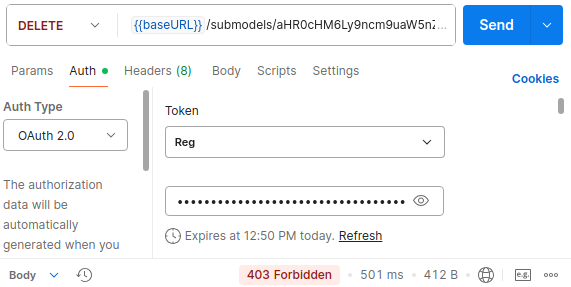
\includegraphics{Bilder/Ergebnisse/DPP/Postman/TechnicianDelet.png}
    \caption{DELETE-Anfrage des Service-Techniker-Clients in Postman}
    \label{fig:KeycloakAnmeldeSeite}
\end{figure}

Abbildung \ref{fig:KeycloakAnmeldeSeite} zeigt eine DELETE-Anfrage, bei der der Service-Techniker-Client versucht, das CF-Submodell aus der AAS-Umgebung zu löschen. 
Da dieser Client lediglich über Leserechte verfügt, wird die Anfrage mit dem HTTP-Statuscode 403 Forbidden abgelehnt.
Wird dieselbe Anfrage hingegen mit dem Groninger-Client ausgeführt, gelingt der Löschvorgang. 
Da dieser über die Rolle Groninger-Mitarbeiter verfügt, besitzt er die erforderlichen Schreibrechte und erhält als Antwort den Statuscode 204 No Content.

Zeigt dass sich differenzierte Zugriffskontrollen auf Submodell-Ebene technisch realisieren lassen.
sensible Informationen verbergen
Die könnte sogar auch noch feingranularer auf Submodelelement Ebene erweitert Wiederverwendung
Dies bietet Potenzial für zukünftige Szenarien, bei denen sensible Nachhaltigkeitsdaten nur bestimmten Akteuren entlang der Wertschöpfungskette zugänglich gemacht werden sollen.

\subsection{Anwendungsfall automatisierte Generierung der AAS}
% \subsection{Einsatzmöglichkeiten von KI im Kontext der Verwaltungsschale}
% \subsubsection{Generierung von Verwaltungsschalen}
% \subsubsection{Anomaliererkennung}
% \subsubsection{Weiterführende Einsatzmöglichkeiten}

%Evaluation der eingesetzten Software
\subsection{Evaluierung eingesetzter Tools und Software}
\subsubsection{Package Explorer}

Der Package Explorer wurde während der gesamten Projektlaufzeit als zentrales Modellierungstool eingesetzt. 
Er diente zur Erstellung, Bearbeitung und Visualisierung der \acs{aas}, einschließlich Submodellen und Concept Descriptions.
Dabei überzeugte das Tool vor allem durch seine benutzerfreundliche und intuitive Oberfläche, welche die Modellierung deutlich vereinfachte. 
So wurden beispielsweise automatische Hinweise gegeben, wenn gegen bestimmte Vorgaben verstoßen wurde, wodurch Fehler frühzeitig erkannt und vermieden werden konnten.

Trotz der zahlreichen positiven Eigenschaften weist der Package Explorer an einigen Stellen noch Mängel in Stabilität und Funktionalität auf. 
Besonders die Validierungsfunktion erwies sich als unzuverlässig, weshalb auch ergänzend externe Testwerkzeuge eingesetzt werden mussten. 
Zudem wird das Tool nicht regelmäßig an neue Versionen der \acs{aas}-Spezifikationen angepasst, was potenziell zu Inkonsistenzen zwischen den Modellen und den Spezifikationen führen kann.



Import von SMT
Vielfältige Exportmöglichkeiten: z.B. AASX-Dateien, JSON, XML.
Verbindung zu AAS Server möglich: Praktisch für lokale Tests und das Verhalten in Laufzeitumgebungen.
Eingabemasken für Concept Descriptions (CD): Strukturierte Erfassung semantischer Informationen.
Direkter Import von ECLASS-Katalogen: Erleichtert semantische Modellierung und Interoperabilität.
copy Refactor: ELemente eines AAS Pakets können kopier tund wiederverwendet werden





Stärken
Benutzerfreundliche Oberfläche: Intuitiv bedienbar, auch für weniger technisch versierte Nutzer.
Komplette Modellierung möglich: Alle Elemente der AAS (Submodelle, Properties, Beziehungen etc.) können erstellt und bearbeitet werden.
Grafische Darstellung: Struktur der AAS ist visuell nachvollziehbar.
Import von Submodel Templates: Erleichtert Standardisierung und Wiederverwendung.
Einfache Einbettung von Dokumenten.
Import von SMT
Vielfältige Exportmöglichkeiten: z.B. AASX-Dateien, JSON, XML.
Verbindung zu AAS Server möglich: Praktisch für lokale Tests und das Verhalten in Laufzeitumgebungen.
Eingabemasken für Concept Descriptions (CD): Strukturierte Erfassung semantischer Informationen.
Direkter Import von ECLASS-Katalogen: Erleichtert semantische Modellierung und Interoperabilität.
copy Refactor: ELemente eines AAS Pakets können kopier tund wiederverwendet werden


Schwächen
Validierungsfunktion unzuverlässig: Nicht vollständig abgestimmt mit externen Tools wie der BaSyx Test Engine.
Nicht alle Funktionen stabil oder vollständig implementiert.
Keine direkte Integration in modulare BaSyx-Umgebung: Verbindung nur zu einem AAS Server möglich. Nicht zu BaSyx weil modular also keinen klassischen Server
Manuelle Bereitstellung notwendig: Für komplexe Szenarien mit mehreren Submodellen oder dynamischen Daten ist zusätzliche Konfiguration erforderlich.
Projektstatus „Incubating“: Tool befindet sich noch in Entwicklung, was zu Änderungen und eingeschränkter Stabilität führen kann.

\subsubsection{Eclipse AASX Server}
\subsubsection{BaSyx}